\documentclass[usenames,dvipsnames]{standalone}
\usepackage{tikz}
\usepackage{tikz-network}
\usepackage{libertine}
\usepackage{libertinust1math}
\usepackage{pgfplots}

\usepackage[T1]{fontenc}
\usetikzlibrary{patterns.meta,decorations.pathmorphing}

\begin{document}
	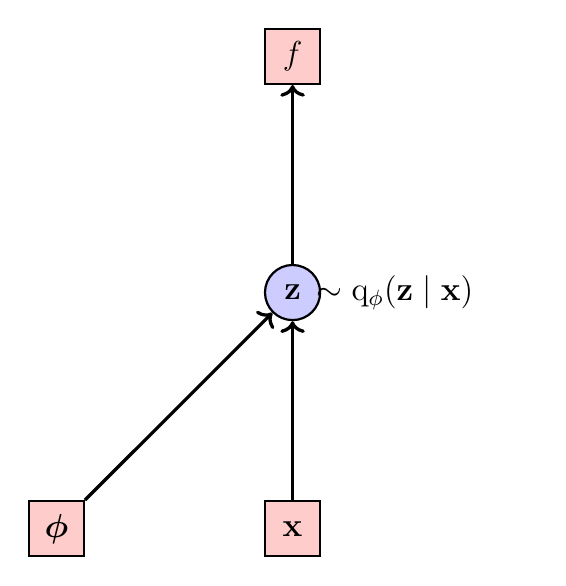
\begin{tikzpicture}
		
		% Original form
		\node[black, style={rectangle, fill=red!20, minimum size = 7mm, draw=black, thick}] (f) at (3, 6) {\large $f$};
		\node[black, style={circle, fill=blue!20, minimum size = 7mm, draw=black, thick}] (z) at (3, 3) {\large $\mathbf{z}$};
		\node[] (samp) at (4.3, 3) {\large $\sim \mathrm{q}_{\phi}(\mathbf{z} \mid \mathbf{x})$};
		\node[black, style={rectangle, fill=red!20, minimum size = 7mm, draw=black, thick}] (x) at (3, 0) {\large $\mathbf{x}$};
		\node[black, style={rectangle, fill=red!20, minimum size = 7mm, draw=black, thick}] (phi) at (0, 0) {\large $\boldsymbol{\phi}$};
		\node[] (ph) at (6, 0) {};
		
		% Connect
		\draw[->, very thick] (phi) -- (z);		
		\draw[->, very thick] (z) -- (f);
		\draw[->, very thick] (x) -- (z);
		
	\end{tikzpicture}
\end{document}